%EE19B070 EE2703 Assignment 3
%this is the symbol for comments in overleaf

\documentclass[11pt]{article}
\usepackage[a4paper,margin=1in]{geometry}
\usepackage{graphicx} %required to load images
\usepackage{amsmath} %required for the matrices
\usepackage{listings}
\usepackage{float}
\usepackage[utf8]{inputenc}
\usepackage{natbib}

\title{EE2703 Assignment3}
\author{Anvith Pabba EE19B070}
\date{5th March 2021}


\begin{document}

\maketitle

\section{Abstract}
This week's Python Assignment focuses on the following topics:
\begin{itemize}
    \item Analysing the data to extract information
    \item Studying the effect of noise on the fitting process
    \item Plotting the relevant graphs
\end{itemize}


\section{Introduction}
Let us model our data in the following form:
\begin{equation*}
g(t) = A*J_2(t) +B*t +n(t)
\end{equation*}
where \begin{textit}A,B\end{textit} are the parameters to be fitted and \begin{textit}J_2(t),t\end{textit} are the given functions in variable \begin{textit}t\end{textit}.
Here,
\begin{itemize}
    \item \begin{textit}A = 1.05\end{textit}
    \item \begin{textit}B = -0.105\end{textit}
    \item \begin{textit}n(t)\end{textit} is the function of the added noise
    \item \begin{textit}J_2(t)\end{textit} is Bessel's function
\end{itemize}

\section{The Assignment}
\subsection{: Generating the data}
We generate the required data by running the \begin{textit}generate\_data.py\end{textit} script. This gives us a \begin{textit}fitting.dat\end{textit} file which contains 10 columns and 101 rows. In this file, the first column is time and the remaining columns are the corresponding data.

\subsection{: Loading the data}
We use the built in \begin{textbf}loadtxt\end{textbf} command that unpacks the fitting.dat (or any given input file) into a new variable, \begin{textbf}data\end{textbf}. This data is loaded column wise.

\subsection{: Defining the function}
We can define the function g(t,A,B) in python using the following snippet:
\begin{verbatim}
def g(t, A, B):
    return A*jn(2,t)+B*t
\end{verbatim}

\subsection{: Plotting the curves:}
We plot the exact value of the function, along with the 9 other noisy plots that we extracted from the generated data. These curves together make up the 'Figure 0' plot.
\subsubsection{: Code Snippet}
We can plot them using the following python code:
\begin{verbatim}
ylabel('$f(t)+noise$',size = 15)
xlabel('$t$',size = 15)
title('Figure 0')
for k in range(9):
	labels = '\u03C3' + subscripts[k] + '=' + str(np.round(sigma[k],3))
	plot(data[0],data[k+1],label = labels)
	legend(loc = 'upper right')
plot(data[0],g(data[0],1.05,-0.105),color = 'black', label = 'f(t)')
legend(loc = 'upper right')
grid(True)
show()
\end{verbatim}

\subsubsection{: Plot of Figure 0}
\begin{figure}[H]
    \centering
    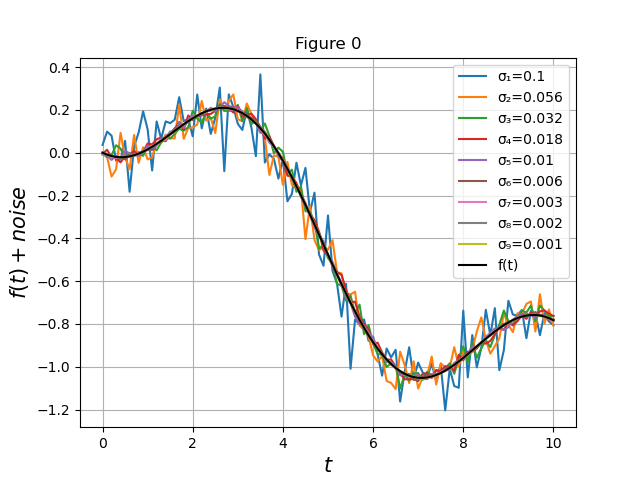
\includegraphics[scale = 0.75]{Figure_1.png}
    \caption{True and noisy plots}
\end{figure}


\subsubsection{: All the different labels}
\begin{itemize}
    \item ylabel, xlabel : these label the y-axis and the x-axis
    \item title : gives a title to the plot
    \item labels : gives a label of each plot that is shown in the legend
    \item color : sets the color of the plot
    \item plot() : is the function used to plot the graph
\end{itemize}

\subsection{: The Errorbars plot}
Plotting the Errorbars gives us a visual representation of the error between a noisy plot and an exact plot. The picture below plots the Errorbar at every 5th data point. 
\subsubsection{: Code Snippet}
\begin{verbatim}
#plotting the errorbar of noise vs time
xlabel('$t$',size = 15)
title('Q5: Data points for \u03C3=0.100 along with the exact function')
errorbar(data[0][::5],data[1][::5],sigma[0],fmt='ro',label='Errorbar') 
#errorbar plot, standard deviation is 0.1 (== sigma[0])
plot(data[0],g(data[0],1.05,-0.105),label = 'f(t)', color= 'black' )
legend(loc = 'upper right')
grid(True)
show()
\end{verbatim}
\subsubsection{: Plot of Errorbars}
\begin{figure}[H]
    \centering
    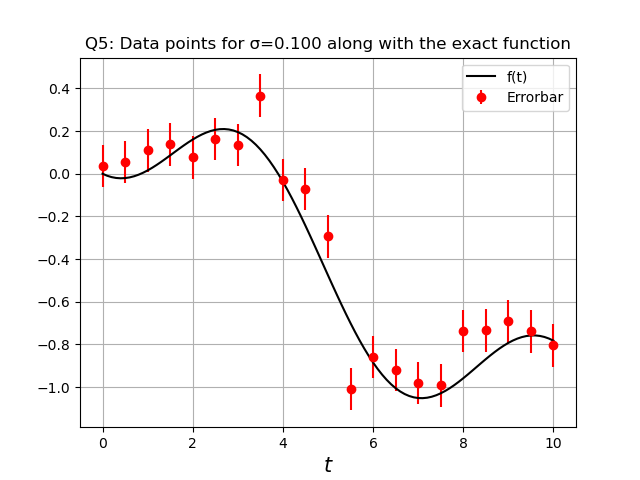
\includegraphics[scale = 0.75]{Figure_2.png}
    \caption{Errorbars plot}
\end{figure}

\subsection{: Creating the required Matrices and checking for equivalence}
We generate 2 matrices, M and p, such that :
\begin{equation}
M = 
\left(\begin{array}{cc} J_2(t_1) & t_1\\ J_2(t_2) & t_2\\... & ...\\J_m(t_1) & t_m \end{array}\right)
\end{equation}
and :
\begin{equation}
p = 
\left(\begin{array}{cc} A\\B \end{array}\right)
\end{equation}
We then find the dot product of M and p and see if that is equal to the values generated from the function g(t,A,B) that we defined before.

\subsubsection{code generating M}
\begin{verbatim}
J = []
for t in data[0]:
J.append(jn(2,t))
M = c_[J,data[0]]
\end{verbatim}
\subsubsection{code generating p}
\begin{verbatim}
A0 = 1.05
B0 = -0.105
p = [[A0],[B0]]
\end{verbatim}

\subsubsection{Checking equivalence of two matrices}
To check the equivalence of the 2 obtained matrices, RHS that we get from g(t,A,B) and LHS from M.p (M dot product with p), I have used the \begin{textbf}array_equal\end{textbf} command in the numpy dictionary. This command return \begin{textbf}True\end{textbf} when both matrices are equal and \begin{textbf}False\end{textbf} when both are not. We then print out the output.

\subsection{Mean squared error and the contour plot}
To check the error between the generated A,B and the exact A,B , we can use the Mean squared error. We calculate the Mean squared error as follows:
\begin{equation}
\varepsilon_i_j &= \sum_{k=0}^{101} (f(k) - g(t_k,A_i,B_j))^2
\end{equation}

\subsubsection{: code}
\begin{verbatim}
for i in range(21):
	for j in range(21):
		for k in range(len(data[0])):
			e[i][j] += (1/101)*((data[1][k]-g(data[0][k],A[i],B[j]))**2)

\end{verbatim}

\subsubsection{: Contour plot}
\begin{figure}[H]
    \centering
    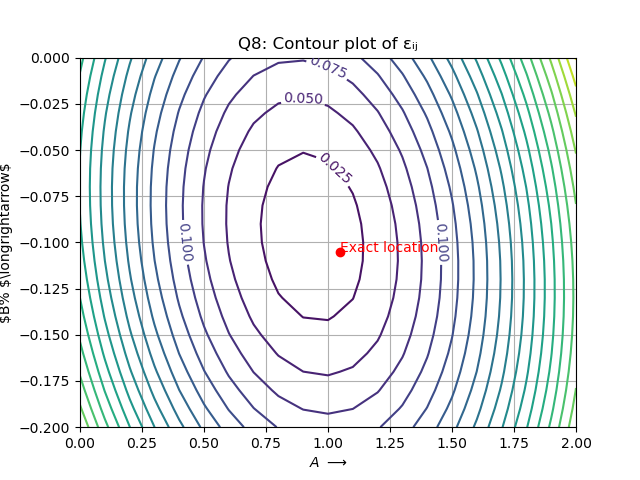
\includegraphics[scale = 0.75]{Figure_3.png}
    \caption{Contour plot of Errors}
\end{figure}

\subsubsection{: Observations}
We can see that there exists only \begin{textbf}1\end{textbf} minimum (we can also see this through the code below which tells us the number of minimums, and as expected, the number of minimums is one) 
\subsubsection{: Code to check number of minimums}
\begin{verbatim}
error_min = 100
for i in range(21):
	for j in range(21):
		if e[i][j] < error_min:
			error_min = e[i][j]
\end{verbatim}

\subsection{Calculating the best fit A and B and plotting the error}
We can find the best fit A and B by minimising,
\begin{equation}
|M.(Aestimate,Bestimate) - (given\_data)|
\end{equation}
To do this, we can use the built in lstsq() function from scipy.linalg which gives us the direct estimates of A and B.

\subsubsection{: Answer to asked question}
From the plot below, it is evident that the graph isn't linear with time. So No, the error does NOT linearly vary with noise.

\subsubsection{: Plot of error of A and B on the linear scale}
\begin{figure}[H]
    \centering
    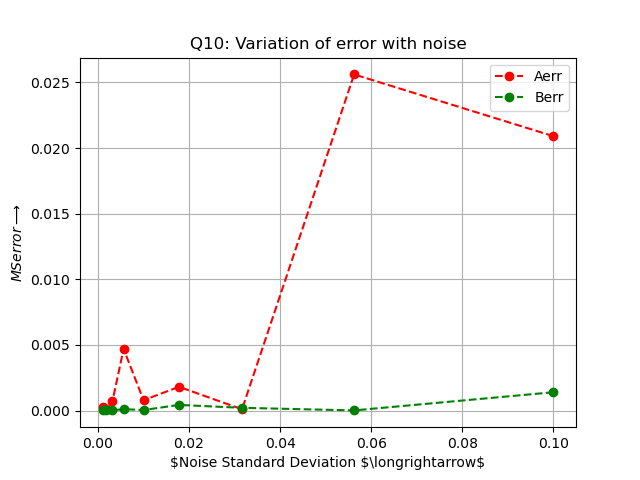
\includegraphics[scale = 0.75]{Figure_4.png}
    \caption{Error of A and B}
\end{figure}

\subsection{Plotting the above error in loglog}
We just plot the same data as above, but we change the scale of the x and y axis to the log scale, by using the xscale and yscale commands

\subsubsection{: Answer to asked question}
In the graph below, we can see that the error is almost linear. In theory, the loglog plot is linear. So Yes, the errors vary linearly in the loglog plot. As the sigma varies exponentially, this linear plot tells us that the noise also increases exponentially.

\subsubsection{: loglog scale plot}
\begin{figure}[H]
    \centering
    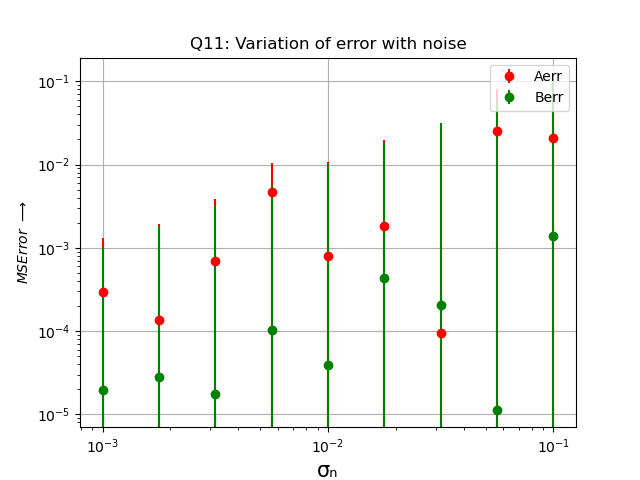
\includegraphics[scale = 0.75]{Figure_5.png}
    \caption{Error of A and B in loglog scale}
\end{figure}

\section{Learning}
What I've learnt from this Assignment.
\begin{itemize}
    \item How to extract data using loadtxt
    \item How to use lstsq to get the best estimates
    \item How to plot various types of graphs and learnt about the various labels that can be manipulated
\end{itemize}

\section{Conclusion}
\begin{itemize}
    \item The error plot of A and B varies linearly in the loglog scale
    \item There is only 1 minima in the contour graph
\end{itemize}

\begin{textbf}\\
\centerline{-THE END-}
\centerline{EE19B070}
\centerline{Anvith Pabba}
\centerline{9381040535}
\end{textbf}








\end{document}
